
\section{Simulation of the DC-DC Buck Converter (Actual Ratings)}
\subsection{Simulation of the DC-DC Buck Converter with Resistive Load}

To validate the dynamic performance and stability of the designed DC-DC buck converter, a high-fidelity simulation model was developed. The system was evaluated under a purely resistive load ($R$-load) across two distinct control configurations: Closed-Loop Current Control and Closed-Loop Voltage Control.

\subsubsection{Simulation Model and Waveform Configurations}

The complete simulation schematic for the DC-DC buck converter configuration under an $R$-load is presented in Figure~\ref{fig:simulink_model_r}.

\begin{figure}[H] 
\centering
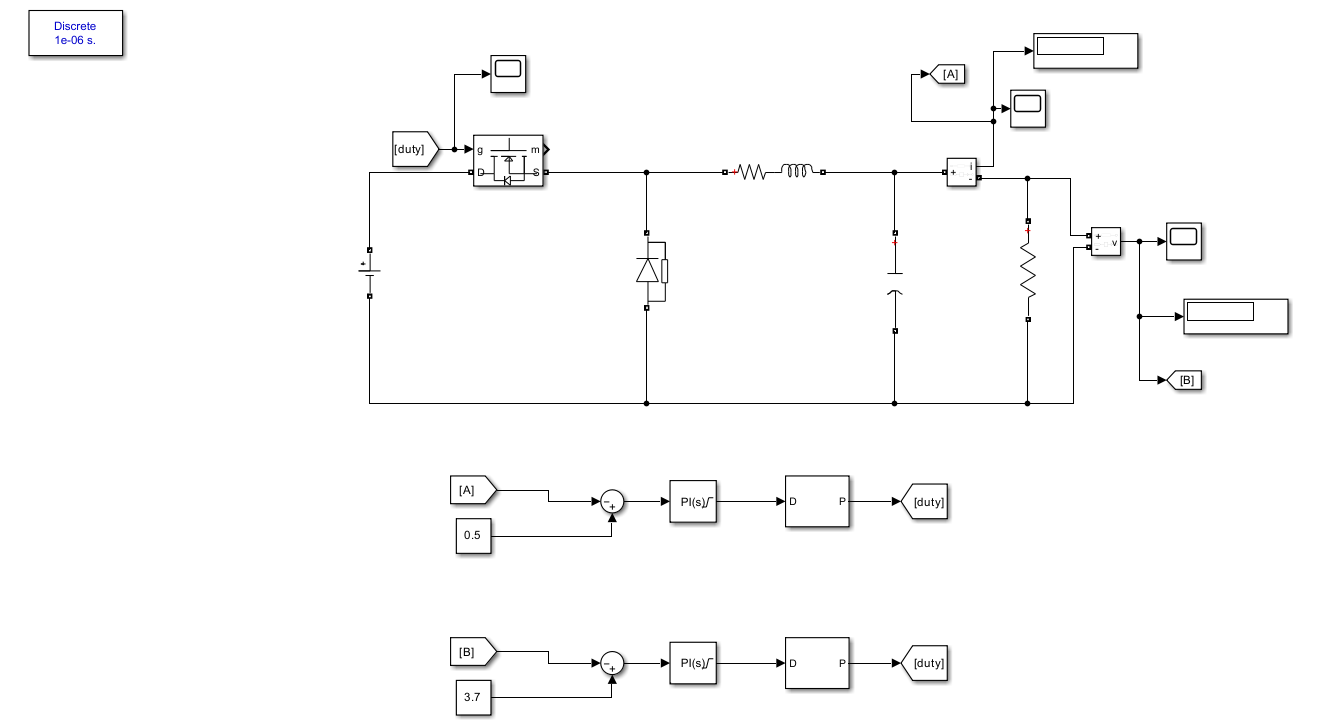
\includegraphics[width=0.9\textwidth]{Figures/buck/buck1.png}  
\caption{Buck converter with an $R$-load configuration simulation model setup.}
\label{fig:simulink_model_r}
\end{figure}

\subsubsection{System Specifications and Model Parameters}
The electrical parameters utilized in the simulation model match the physical component characteristics of the prototype implementation. These parameters are summarized in Table~\ref{tab:buck_parameters}.

\begin{table}[H] 
\centering
\caption{DC-DC Buck Converter Simulation Parameters}
\label{tab:buck_parameters}
\begin{tabular}{lcc}
\hline
\textbf{Parameter} & \textbf{Symbol} & \textbf{Value} \\ \hline
Input Voltage & $V_{\text{in}}$ & 12.3~V \\
Filter Inductance & $L$ & 2~mH \\
Inductor Internal Resistance & $R_L$ & 1.9~$\Omega$ \\
Filter Capacitance & $C_{\text{out}}$ & 220~$\mu$F \\
Resistive Load & $R$ & 10~$\Omega$ \\
Switching Frequency & $f_{sw}$ & 10~kHz \\
Simulation Time Step (Discrete) & $T_s$ & 1~$\mu$s \\ \hline
\end{tabular}
\end{table}

The internal resistance of the inductor ($R_L = 1.9~\Omega$) was explicitly included in the simulation to account for realistic conduction losses and to accurately evaluate the damping behavior of the plant during transients.

\subsubsection{Control Architecture}
Proportional-Integral (PI) controllers were chosen to eliminate steady-state error and achieve the desired transient tracking. The controller gains were derived using the control design discussed in chapter 4 tuned specifically to match the transfer function of this hardware configuration at an operating frequency of 10~kHz. 

The control framework evaluates two operating scenarios independently, where the generated control signal adjusts the duty cycle ($D$) fed to the MOSFET gate driver via a Pulse Width Modulation (PWM) block:

\begin{enumerate}
    \item \textbf{Current Control Loop:} The inductor current $i_L$ is subtracted from a reference current command of 0.5~A. The tracking error processed by the PI controller is formulated as:
    \begin{equation}
    e_i(t) = 0.5 - i_L(t)
    \end{equation}
    
    \item \textbf{Voltage Control Loop:} The output voltage $v_{\text{out}}$ across the 10~$\Omega$ load resistor is compared against a reference voltage command of 3.7~V. The error signal is formulated as:
    \begin{equation}
    e_v(t) = 3.7 - v_{\text{out}}(t)
    \end{equation}
\end{enumerate}

\subsubsection{Simulation Results and Discussion}
The discrete-time solver was executed with a fixed time step of 1~$\mu$s over a total duration of 4~seconds, yielding exactly 100 simulation samples per 10~kHz switching period ($T_{sw} = 100\ \mu$s).
\newpage
\paragraph{Closed-Loop Current Control Response}
When operating under current control with a step reference of 0.5~A, the system exhibits a highly damped, stable transient response. As illustrated in the simulation scope output in Figure~\ref{fig:current_loop_res}, the current rises smoothly without visible overshoot. It exhibits a slight stair-step behavior during the initial startup phase—a direct result of the discrete control loop updates interacting with the inductor time constant ($\tau = L/R_L \approx 1.05$~ms)—before settling precisely at 0.5~A within approximately 0.4~seconds. The steady-state ripple is tightly bounded, indicating optimal tuning of the current loop PI parameters at this switching frequency.

\begin{figure}[H] 
\centering
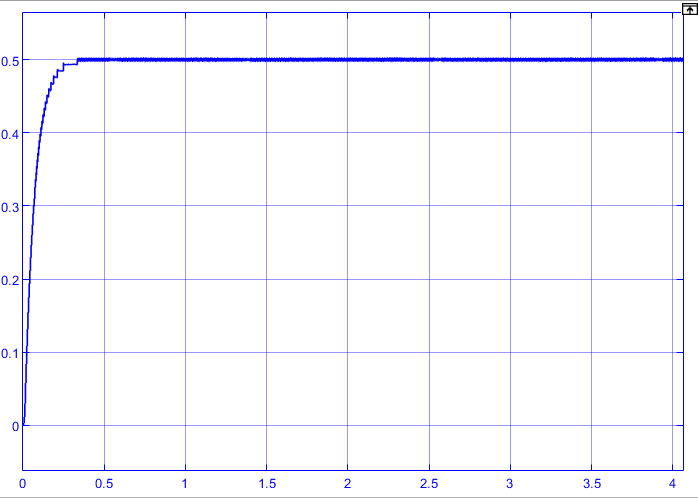
\includegraphics[width=0.75\textwidth]{Figures/buck/current1.png}  
\caption{Current control closed-loop transient response ($i_o$ vs. time) reaching a steady state of 0.5~A.}
\label{fig:current_loop_res}
\end{figure}

\paragraph{Closed-Loop Voltage Control Response}
For the voltage control validation, the reference command was set to 3.7~V. The corresponding output voltage waveform shown in Figure~\ref{fig:voltage_loop_res} shows an exceptionally fast transient response. The voltage climbs sharply at $t = 0$~s with a negligible overshoot of approximately 2.7\% (peaking briefly at $\approx 3.8$~V) before fully settling to the target 3.7~V in under 0.05~seconds. The minimal steady-state voltage ripple underscores the effective high-frequency filtering provided by the 220~$\mu$F output capacitor against the 10~kHz switching harmonics.

\begin{figure}[H] 
\centering
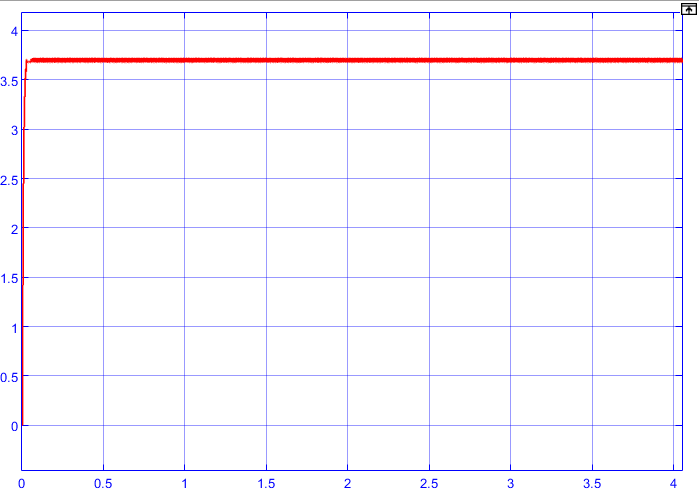
\includegraphics[width=0.75\textwidth]{Figures/buck/volt1.png}  
\caption{Voltage control closed-loop transient response ($v_{\text{out}}$ vs. time) reaching a steady state of 3.7~V.}
\label{fig:voltage_loop_res}
\end{figure}


\subsection{Simulation of the DC-DC Buck Converter with RC load representing Lithium-Ion Battery}

To evaluate the converter performance under realistic energy storage conditions, the resistive load was replaced with an equivalent model of a Lithium-ion (Li-ion) battery. A common method for macro-level dynamic simulation represents the battery using a series resistance-capacitance ($RC$) network. 

\subsubsection{Battery Specifications and Modeling Parameters}
The target energy storage element is a standard $3.7\text{ V}$, $800\text{ mAh}$ Li-ion cell. To capture the long-term voltage charging dynamics alongside high-frequency power stage interactions within a reasonable simulation timeframe, the parameters were extracted using fundamental energy capacity relations. The total nominal charge capacity in Coulombs ($Q$) is calculated as:
\begin{equation}
Q = 0.8\text{ Ah} \times 3600\text{ s/h} = 2880\text{ C}
\end{equation}

Assuming a standard $1\text{ V}$ usable voltage delta across the linear state-of-charge region, the equivalent capacitance ($C_{\text{batt}}$) is modeled as $2880\text{ F}$. The internal cell ohmic losses are modeled via a series internal resistance ($R_{\text{batt}}$) of $0.1\ \Omega$. The complete simulation configuration schematic containing this $RC$ network is illustrated in Figure~\ref{fig:simulink_model_battery}.

\begin{figure}[H] 
\centering
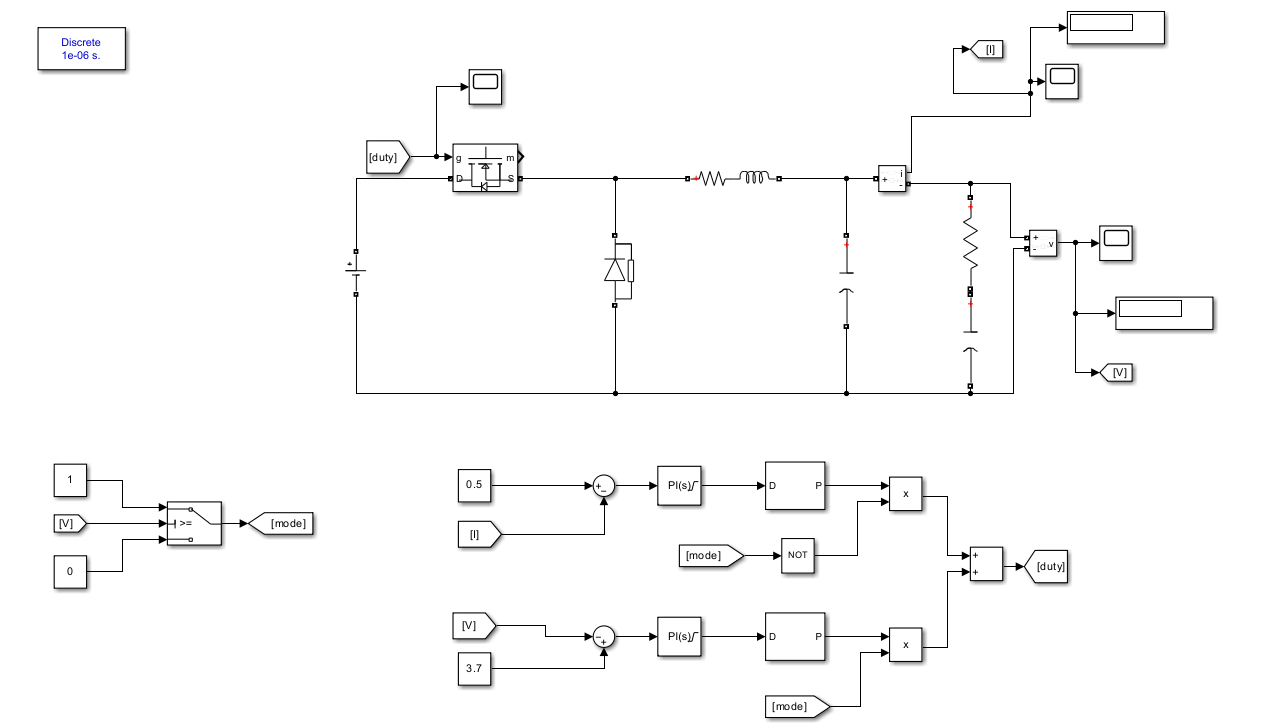
\includegraphics[width=0.9\textwidth]{Figures/buck/buck2.png}  
\caption{Setup for the buck converter operating with an equivalent $RC$ Li-ion battery load.}
\label{fig:simulink_model_battery}
\end{figure}

\begin{table}[H] 
\centering
\caption{DC-DC Buck Converter Simulation Parameters}
\label{tab:buck_parameters}
\begin{tabular}{lcc}
\hline
\textbf{Parameter} & \textbf{Symbol} & \textbf{Value} \\ \hline
Input Voltage & $V_{\text{in}}$ & 12.3~V \\
Filter Inductance & $L$ & 330~$\mu$H \\
Inductor Internal Resistance & $R_L$ & 0.1~$\Omega$ \\
Filter Capacitance & $C_{\text{out}}$ & 220~$\mu$F \\
Load Resistance & $R_L$ & 0.1~$\Omega$ \\
Load Capacitance & $C_L$ & 2880~$\Omega$ \\
Switching Frequency & $f_{sw}$ & 10~kHz \\
Simulation Time Step (Discrete) & $T_s$ & 1~$\mu$s \\ \hline
\end{tabular}
\end{table}

\subsubsection{Control Framework and Mode Control Logic}
Unlike the standard independent loops utilized for the resistive load, the battery charging control architecture utilizes automated loop arbitration based on a dynamic logic mode switch block:
\begin{enumerate}
    \item \textbf{Constant Current (CC) Charging Stage:} When the battery voltage is below a threshold or during initial high-current demands, the controller tracks a target current reference of $0.5\text{ A}$ via the inductor current feedback loop tag \texttt{[I]}.
    \newpage
    \item \textbf{Constant Voltage (CV) Charging Stage:} As the battery voltage tag \texttt{[V]} builds up and approaches the set boundary condition, a conditional logic block ($[V] \ge 3.7$) triggers a mode state change switch, overriding the current loop and passing the output of the $3.7\text{ V}$ voltage tracking PI controller to the duty cycle generation port.
\end{enumerate}

\subsubsection{Simulation Results and Discussion}
The model was compiled under a discrete execution step size of $T_s = 1\ \mu\text{s}$ at a fixed $10\text{ kHz}$ switching frequency.

\paragraph{Battery Charging Current Profile}~\hfill\\
The transient current response during the constant current mode tracking is shown in Figure~\ref{fig:battery_current_res}. 

\begin{figure}[H] 
\centering
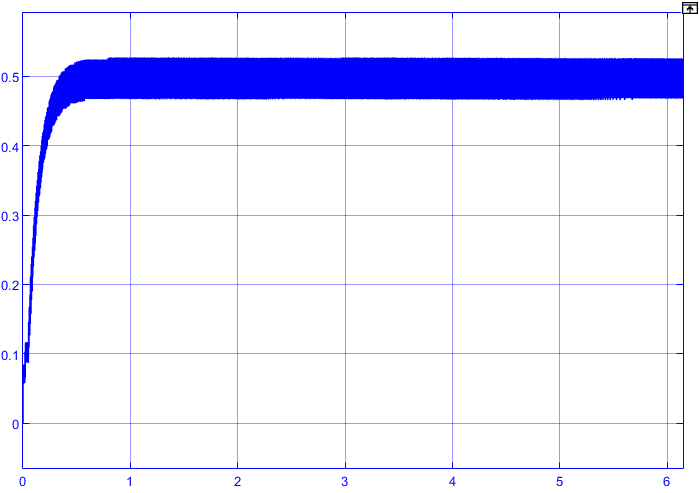
\includegraphics[width=0.75\textwidth]{Figures/buck/current2.png}  
\caption{Closed-loop battery current response.}
\label{fig:battery_current_res}
\end{figure}

The current displays a highly damped rise time, stabilizing safely at the targeted current range within approximately $0.5\text{ seconds}$. Because of the very low damping properties of the large capacitance and the $0.1\ \Omega$ battery internal resistance, a dense switching ripple envelope is observed around the steady-state tracking path, showing the demanding requirements placed on the filtering stage under electrochemical loads.

\paragraph{Battery Charging Voltage Profile}~\hfill\\
The battery terminal voltage response under closed-loop control is displayed in Figure~\ref{fig:battery_voltage_res}.

\begin{figure}[H] 
\centering
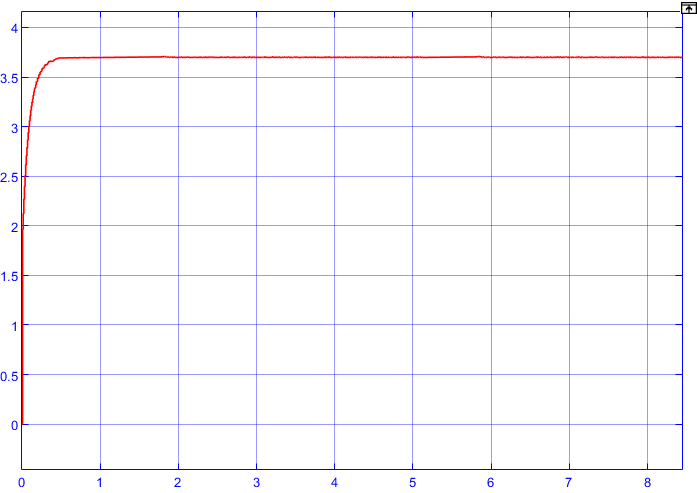
\includegraphics[width=0.75\textwidth]{Figures/buck/volt2.png}  
\caption{Closed-loop battery terminal voltage charging transient settling exactly at $3.7\text{ V}$.}
\label{fig:battery_voltage_res}
\end{figure}

The output voltage rises smoothly from $0\text{ V}$ at startup, experiencing a highly controlled over-damped trajectory that eliminates hazardous voltage overshoots entirely. The voltage settles smoothly at the nominal value of $3.7\text{ V}$ within $0.5\text{ seconds}$ and is held tightly with negligible steady-state ripple, proving the robustness of the PI control system when operating with highly capacitive energy systems.